% Setup - do not change
\documentclass[11pt]{article}
\usepackage[top=0.9in, left=0.9in, bottom=0.9in, right=0.9in]{geometry} 
\usepackage{parskip}
\usepackage{graphicx}

\usepackage[english]{babel}
\usepackage[utf8]{inputenc}
\usepackage{amsmath,amsthm,amssymb,graphicx,pdfpages,lipsum,hyperref}
\usepackage[none]{hyphenat}
\usepackage{csquotes}
\usepackage{adjustbox}
\usepackage{caption}
\usepackage{subcaption}
\usepackage{amsmath}
\usepackage{listings}
\lstset{
    language=Python, % Set the programming language
    basicstyle=\ttfamily, % Set the font style for code
    keywordstyle=\color{blue}, % Set color for keywords
    commentstyle=\color{green!40!black}, % Set color for comments
    stringstyle=\color{red}, % Set color for strings
    numbers=left, % Display line numbers
    numberstyle=\tiny\color{gray}, % Style for line numbers
    stepnumber=1, % Increment for line numbers
    tabsize=4, % Set tab size
    showstringspaces=false, % Don't show spaces in strings
    breaklines=true % Allow code to break across lines
}



\setlength\parindent{0pt}
%%%%%%%%%%%%%%%%%%%%%%%%%%%%%%%%%%%%%%%%%%%%%%%%%%%%%%%%%%%%%%%%%%%
% add other packages here if required

%% Bibliography are specified in this file. You can also choose inline bib style if you want to. But make sure your citation style is consistent (and proper)
% For more details on citation: https://library.unimelb.edu.au/recite
\usepackage[sorting = none]{biblatex}
\addbibresource{references.bib}

%%%%%%%%%%%%%%%%%%%%%%%%%%%%%%%%%%%%%%%%%%%%%%%%%%%%%%%%%%%%%%%%%%% the '%' symbol denotes comments

% Begin document creation
% DELETE THE \lipsum PLACEHOLDERS WHEN YOU BEGIN
\title{\textbf{Time series forecasting for Yellow Taxi in New York Inner Urban Boroughs}}
\author{
Ngoc Duy Tran \\
Student ID: 1156724 \\
%% Replace the link with your github repo
% 1. Remember to escape underscore (\_) in the link.
% 2. Remember to include the commit you want to submit in the link
\href{https://github.com/MAST30034-Applied-Data-Science/mast30034-project-1-dduygaucho.git}{Github repo}
}

\begin{document}
\maketitle

\section{Introduction}
% Link to a 30 min tutorial if you require revision: https://www.overleaf.com/learn/latex/Learn_LaTeX_in_30_minutes
Conventional yellow taxi in New York City is currently facing challenges due to the thriving of technologically-driven ride-hailing services like Uber, Grab, and Lyft. Therefore, there exists a substantial demand for taxi companies such as TLC to strategically re-allocate their taxi drivers to specific highly-demanded areas at different times during the day to maximize profit.

\subsection{Research focus}

This research focuses on hourly prediction for highly-demanded taxi boroughs to help the target audience \textbf{TLC} answer a million-dollar question: \textit{Given the data in a borough from the previous w = 96 hours, what are the predictions for yellow taxi demand in the next k = 8 hours?} This research focuses on \textbf{Yellow Taxis} due to its flexibility, in which they have no restrictions in picking up, including Manhattan, the core borough of this study. 
\subsection{Dataset}
The major dataset is \textbf{TLC Taxi Trip Record Data}, capturing taxi ridership features namely pick-up and drop-off locations \cite{NYC-TLC}. Additionally, this research confines the timeframe from 2022 February to 2023 February, ending up with a dataset of 43,172,888 instances and 19 features. Data before February 2022  was also excluded, attributed by a major surge in COVID-19 cases and fatalities, preventing this data from capturing the genuine underlying pattern in taxi ridership demand \cite{NYT-Covid}.

Two external datasets integrated in modelling process are \textbf{MTA Subway Hourly Ridership} \cite{MTA-Ridership} and \textbf{Global Hourly Integrated Surface Database} \cite{NCEI-Surface}. The former dataset presents subway ridership estimates in hourly interval in various boroughs starting from February 2022 with 5,423,857 records and 11 features. Furthermore, the latter dataset incorporates hourly records measured from JFK International Airport from 2022 (13,344 records and 100 features) and 2023 (8475 records and 95 features). More information about these 3 datasets and preprocessing steps will be introduced in Section 2. 
% The shape for 3 datasets is summarized in the following Table \ref{tab:datasets}:

%Therefore, this dataset contains  highly useful features for predicting hourly taxi demand such as $ridership$ (total number of riders entering the station) and $borough$ to which the station belongs. 

 % encompassing attributes like $temperature$ and $wind$, which could potentially serve as an useful predictors for taxi demand patterns as commuters' behaviour for taxi hailing is highly likely influenced by these factors.




% \begin{table}[ht]
% \centering
% \begin{tabular}{|l|l|l|}
% \hline
% \textbf{Datasets}                             & \textbf{Records} & \textbf{Features}    \\
% \hline
% TLC Yellow Taxi Dataset     & 43,172,888 &  19             \\
% Hourly Integrated Surface Database 2022      & 13,344 & 100              \\
% Hourly Integrated Surface Database 2023      & 8,020 & 95              \\
% MTA Subway Dataset      & 5,423,857 & 11                \\
% \hline
% \end{tabular}
% \caption{Summary of Datasets}
% \label{tab:datasets}
% \end{table}

\section{Preprocessing}
\subsection{Landing layer to Raw layer}
After all datasets and supplementary datasets (taxi zone lookup and shape files) are downloaded into the landing layer, the three primary datasets undergo data parsing to ensure consistent data types.

% For the purpose of modelling and analysis, relevant features are preserved across all three datasets. Within Integrated Surface Database, $date$, $wind$, $temperature$ features are retained, while in MTA Subway datasets, $transit\_timestamp$, $borough$, $ridership$ are preserved for taxi demand prediction. However, in the interest of effective data wrangling, TLC Yellow Taxi Dataset preserves all of its attributes to facilitate filtering invalid records.

\subsection{Raw layer to Curated Layer}

\subsubsection{TLC Trip Record Data}
Having inspected the dataset, the dataset comes with a few different problems requiring further filtering and analysis.

\begin{itemize}
    \item \textbf{Filtering records not in the defined timeframe:} Dataset shape: (43172300,19) 
    \item \textbf{Filtering trips with short distance:} Records where trip distance falls below 0.4 miles (~500 meters) are excluded as a discerning passengers would not typically opt for a taxi when the travel distance is below 500 meters. (41811443, 19)
    \item \textbf{Filtering trips with short commuting time 60 seconds:} It would be unreasonable to finish the whole trip under a minute. An extra column is created to find the difference (41753931, 20)

    \item \textbf{Filtering trips with long commuting time 4 hours:} The two furthest locations in New York City is Floral Park and The Conference House, which results in only 45 miles and nearly 2 hours if taken by cars according to Google Maps. The threshold is set at 4 hours in case there is a return. (41704217, 20)
    
    \item \textbf{Filtering trips with long distance:} Records where trip distance exceeds 100 miles are excluded, which doubles the distance from Floral Park to Conference House. (41702718, 20)


    \item \textbf{Filtering trips with fare amount exceeds \$300:} With current choice of maximum trip distance of 100 miles and average price per mile of \$3. (41504885, 20)

    \item \textbf{Filtering trips with pickup locations within New York City:} For visualization, all trips with pick-up location ID outside the range [2-263] are removed. An extra column indicating borough is added. Newark Airport is also excluded because it is not the target of the study, inner-city boroughs (40984627, 21)
     % For modelling, all trips with pick-up location ID = 1 (Newark International Airport) will also be removed because of the focus on 5 boroughs within the city only
    
\end{itemize}

 % As the focus of this project is on predicting the hourly demand for taxi in highly-demanded boroughs, further filtering regarding money including tips, tolls, airport\_fee, etc are not necessary as our model would not be sensitive to these filtering. Nevertheless, with the current filtering design, outliers such as fare amounts or trip distance with 6 significant figures have already been omitted.

 \subsubsection{Hourly Integrated Surface Database}

 The \textcolor{blue}{2022} and \textcolor{red}{2023} weather datasets undergo the process of data wrangling and feature selection. 

 \begin{itemize}
     \item \textbf{Feature selection:} \texttt{date}, \texttt{temperature} and \texttt{wind}, are preserved. \textcolor{blue}{(13344,3)}, \textcolor{red}{(8475,3)}

      \item \textbf{Outlier filtration:} This involves removing outliers for 2 features (denoted as 9999 according to data dictionary) and instances with unqualified quality to avoid any miscalculations. \textcolor{blue}{(12967,3)}, \textcolor{red}{(8235,3)}

     \item \textbf{Merging:} Having been aggregated hourly, both 2022 and 2023 weather datasets are joined with an extra feature created \texttt{hour} for joining.  (\texttt{year\_month\_date}, \texttt{hour}, \texttt{avg\_tmp\_observation}, and \texttt{avg\_speed}) \textcolor{blue}{(8760,4)}, \textcolor{red}{(5528,4)}

      \item \textbf{Timeline filtering:} Both datasets are refined to the specific timeframe ranging from 01/02/2022 to 28/02/2023, \textcolor{blue}{(8016,4)}, \textcolor{red}{(1416,4)}, resulting in a final weather dataset with 9432 instances and 4 features in total
     
 \end{itemize}

 % Given that the data contains multiple records across various minutes within an hour, the fact that we aggregate hourly does not result in missing data.   

 \subsubsection{MTA Subway Hourly Ridership}

 The MTA Subway hourly Ridership undergoes a similar process of data wrangling

 \begin{itemize}
     \item \textbf{Feature selection:} 3 relevant features, namely \texttt{transit\_timestamp}, \texttt{borough} and \texttt{ridership}, are preserved. (5423857, 3) 
     \item \textbf{Timeline filtering:} The dataset is refined to the pre-chosen timeframe. (3913645, 3) 

     \item \textbf{Outlier filtration:} The maximum hourly \texttt{ridership} is 999, which is found in Manhattan and queens boroughs. However, this number is within the expected range as both boroughs often experience ridership around 900 during rush hours. (3913645, 3) 

     \item \textbf{Aggregation and Borough filtering:} The data is then aggregated based on \texttt{borough} and \texttt{transit\_timestamp}.  4 separate datasets are subsequently stored for 4 unique boroughs: Queens, Manhattan, Brooklyn, and Bronx (9432,3)

     % \item \textbf{Missing value imputation:} All 4 borough datasets observe a similar pattern when there is only 1 out of 9432 instances that is missing, which is 2022-03-13 02:00:00. Therefore, this could be due to a systematic error in which the system fails to capture information for this timestamp. In response, linear interpolation is utilized for imputation
 \end{itemize}


 % \subsubsection{Joining 3 major datasets}
 For TLC Trip Record Data, 4 inner-city boroughs are aggregated and saved separately, before joining with MTA Subway and Integrated Surface Database on the timestamp to produce 4 other datasets ready for modelling (9432 instances, 5 features).
 
 % Due to limitations in computational resources and the scope of this study on highly-demanded zones, this research's modelling section covers Queens and Manhattan boroughs only.

\section{Geospatial Visualisation and Feature Analysis}
For \textbf{Section 3 Visualization and Feature Analysis}, this research covers highly-demanded boroughs with a focus on Manhattan; while \textbf{Modelling Section 4} only covers Manhattan time series forecasting due to computational limitations. 
Newark Liberty International Airport is not within the 5 boroughs; therefore, will not be covered in the analysis. 
\subsection{Geospatial visualization}
% \begin{figure}[ht]
%     \centering
%     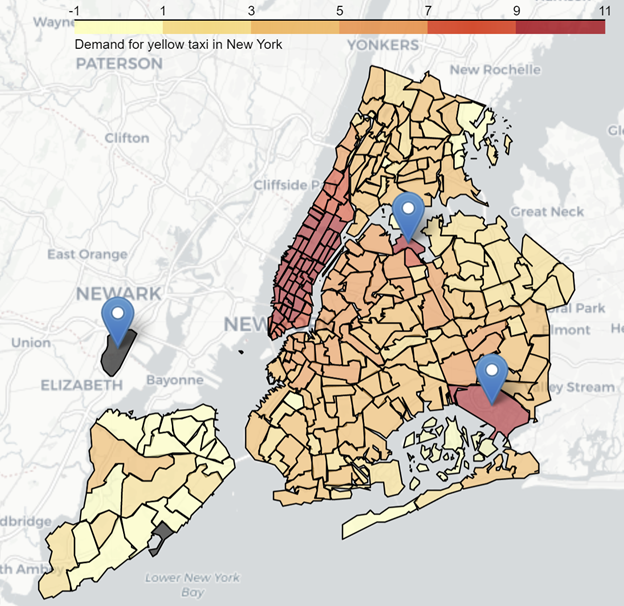
\includegraphics[width=0.5\textwidth]{plots/yellow taxi constant.png}
%     \caption{Hourly demand for Yellow Taxi from February 2022 - February 2023}
%     \label{fig:yellow subway constant}
% \end{figure}


\begin{figure}[ht]
    \begin{minipage}{0.5\linewidth}
        \begin{adjustbox}{left}
            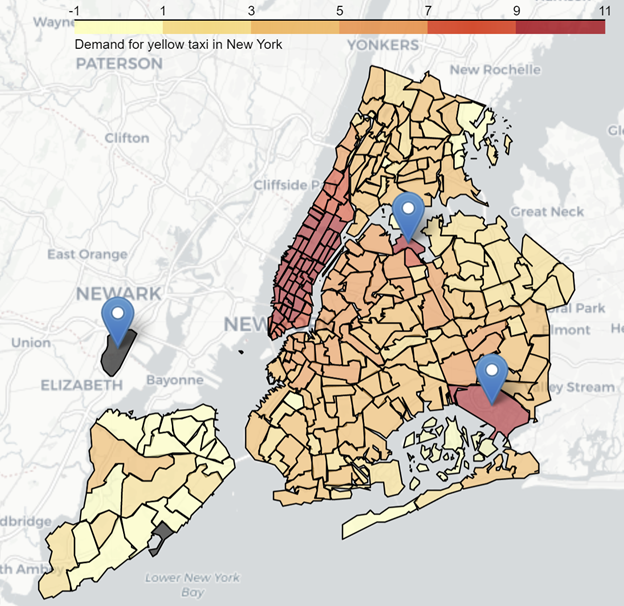
\includegraphics[width=\textwidth]{plots/yellow taxi constant.png}
            
        \end{adjustbox}
    \end{minipage}
    \begin{minipage}{0.5\linewidth}
From Figure \ref{fig:yellow subway constant}, Manhattan, JFK International Airport, and Laguardia Airport stand out as regions with enormous demand for yellow taxis; thereby, attracting an influx of yellow taxi drivers. Therefore, it would be reasonable for TLC to distribute their yellow taxi drivers in proximity to these locations because demand for yellow taxi in areas adjacent to these 3 major hotspots is still high.

On the other hand, Staten Island observes the lowest demand for yellow taxis among the 5 boroughs, which is reasoned by several factors, including higher prevalence of other taxi brands namely Clove Lake Cars and small population (493,194 in Staten Island vs 1,628,706 in Manhattan). 
    \end{minipage}
        \caption{Log Hourly demand for Yellow Taxi from February 2022 - February 2023}
    
    \label{fig:yellow subway constant}
\end{figure}



\subsection{Geospatial visualization across different times during the day}
Figure \ref{fig:geospatial time}a at 2AM presents findings partially aligning with Figure \ref{fig:yellow subway constant}. Though JFK remains highly demanded, it reveals that Laguardia Airport's demand diminishes and Manhattan's demand has now condensed into the downtown and midtown area. These insights could act as TLC's strategy to navigate their yellow taxi drivers to JFK and particularly midtown Manhattan where the profit remains significant, nearly 10,000 rides for a zone at 2 AM. However, not all parts of lower Manhattan are equally busy, illustrated by the \textcolor{red}{red box} in Figure \ref{fig:geospatial time}a. This will be shortly be explained in the next paragraph and followed up in Section 6 Recommendations. Additionally, demand is little outside lower Manhattan and surrounding neighbours, especially in Staten Island, with many zones with no trips recorded (grey).


\begin{figure}[ht]
    \centering
    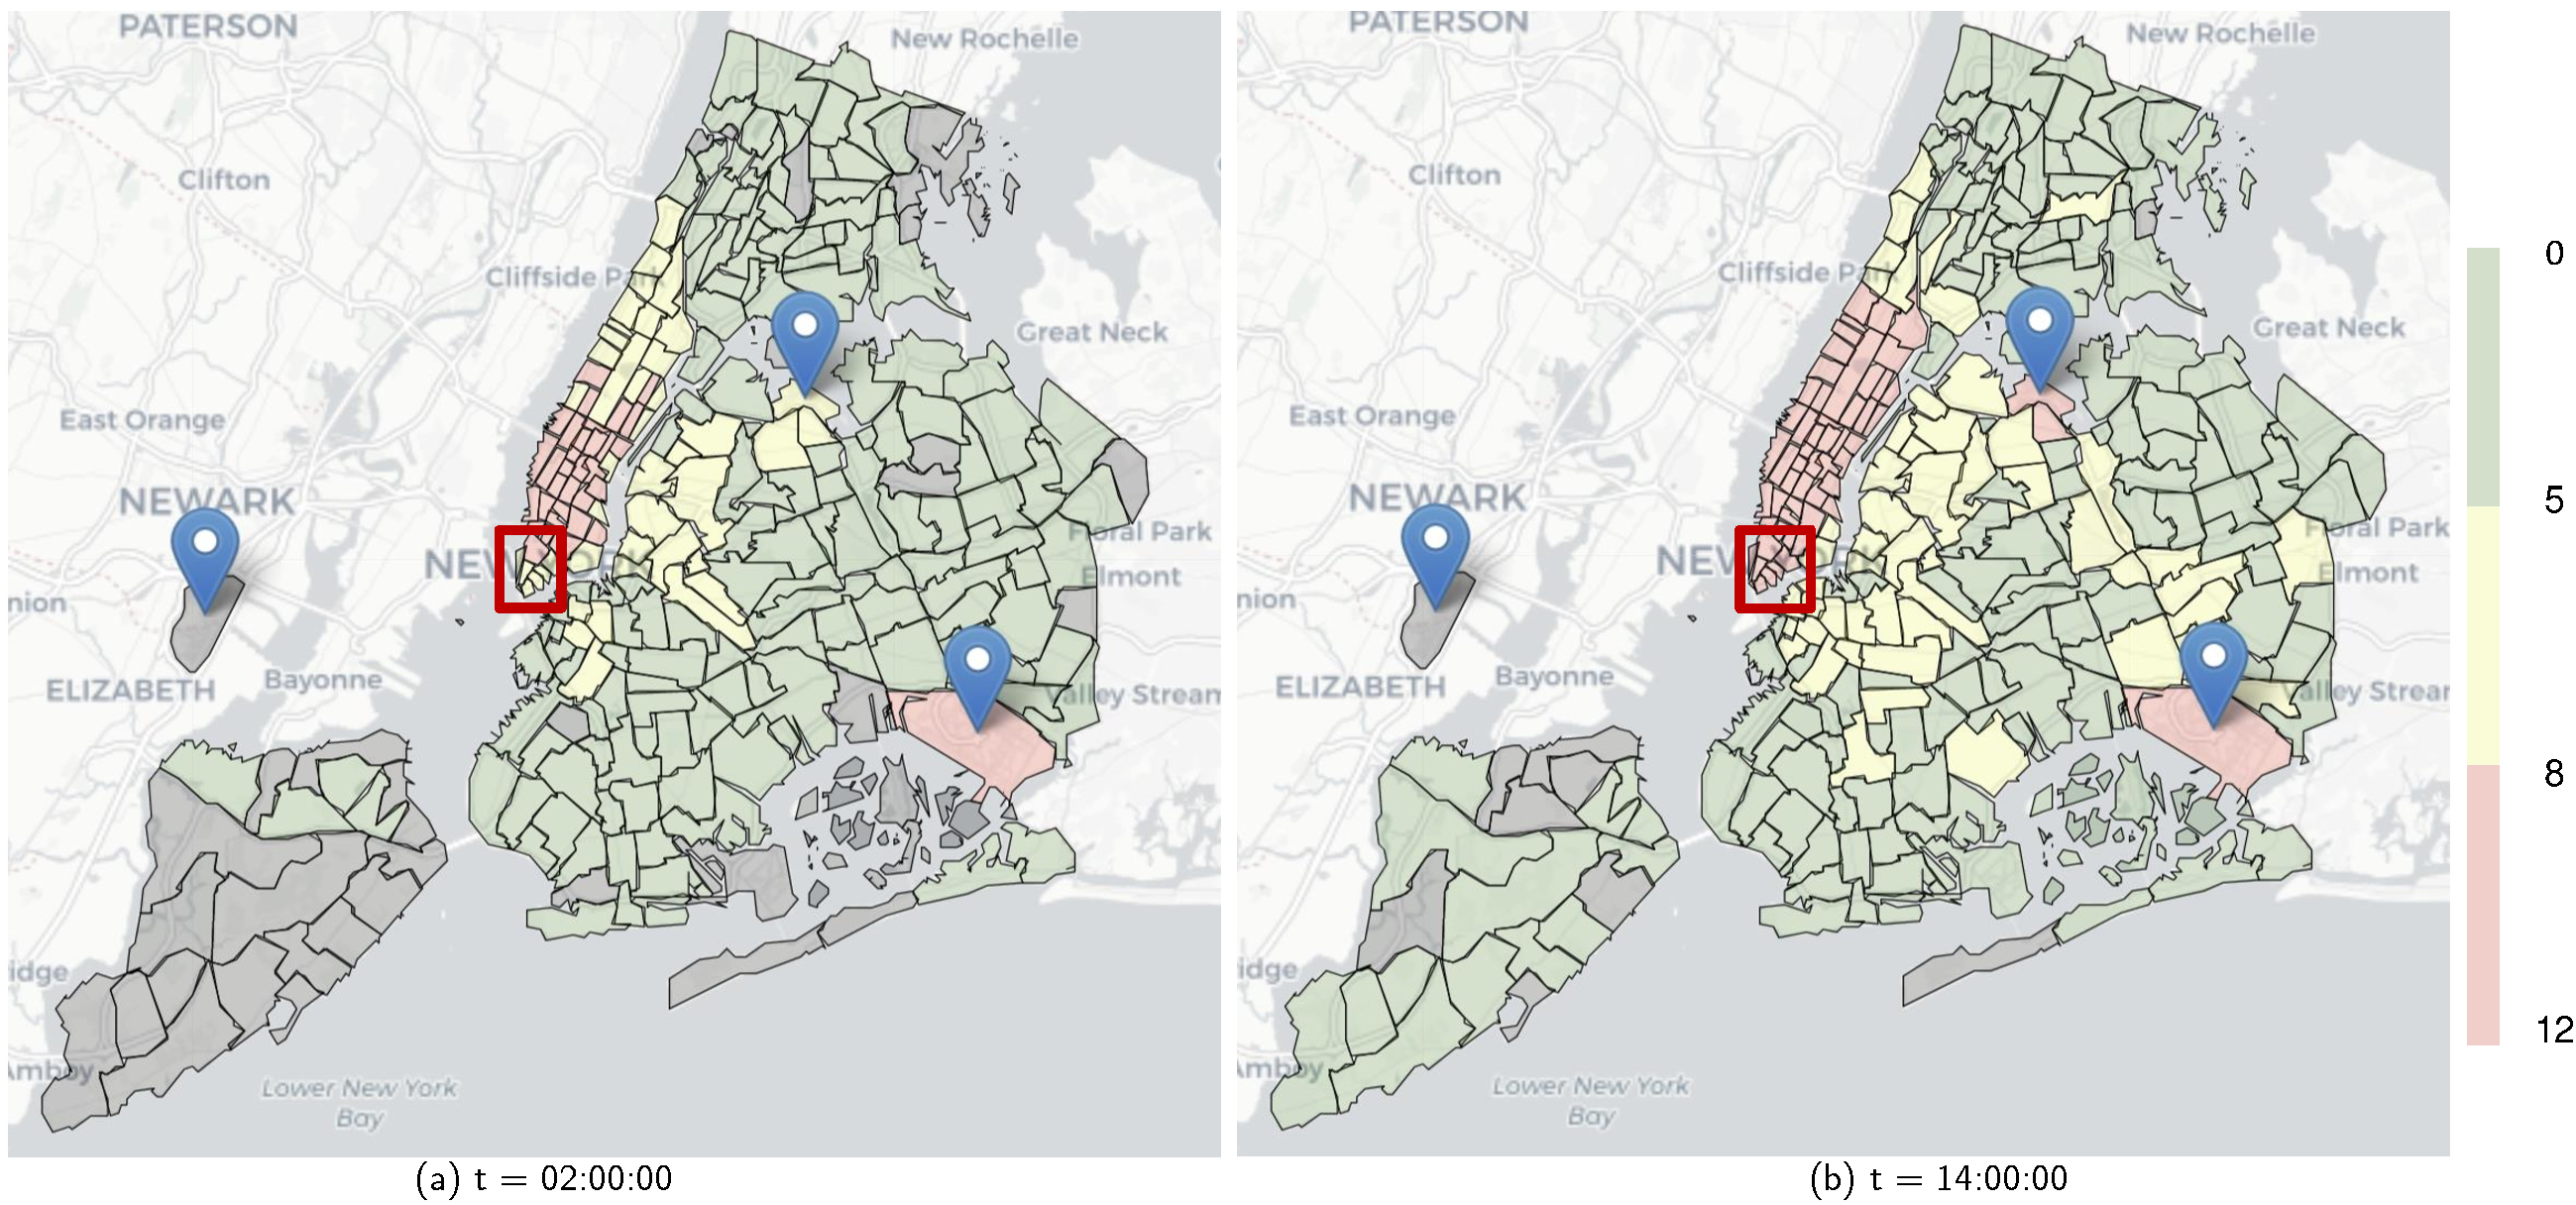
\includegraphics[width=1.0\textwidth]{plots/Figure 1.pdf}
    \caption{Log Hourly demand for Yellow Taxi across different hours}
    \label{fig:geospatial time}
\end{figure}

Figure \ref{fig:geospatial time}b shows while there are discrepancies in 2AM findings, the geospatial demand findings at 14:00 is consistent with results in section 3.1. An interesting observation is that the \textcolor{red}{red box} is heavily demanded 12 hours later. This observation is because red-box region comprises of the Financial District experiencing a major surge in working commuting activities. This is further supported by the region's hosting of various tourist attractions, including Statue of Liberty cruises, attracting many taxi drivers around to transport tourists. Therefore, TLC should encourage their yellow taxi drivers towards lower Manhattan during this period to accommodate the elevated demand, while allocating green taxis to other boroughs to achieve maximum profit.
 % Opposite to 2AM demand, there are now a few taxi drivers in Staten Island, showing there is a transition from Manhattan to Staten Island after 12 hours, yet very small compared to the Central of New York City.
\subsection{Feature analysis}
Firstly, from Figure \ref{subfig:mta_taxi}, there is a positive correlation between \texttt{hourly subway ridership} and \texttt{hourly yellow taxi demand} - response variable. Despite certain differences in the mid-day pattern, both features exhibit similar pattern in the early and late parts. They both show a decreasing trend in demand from 6P.M until 5 A.M in the following day, followed by a spike due to substantial demand for means of transportation during work commutes. This finding is further supported by Figure \ref{subfig:plot2}, revealing a Pearson correlation of 0.8 between these 2 features for the Manhattan borough. These 2 evidence signals the significance of \texttt{hourly subway ridership} as a powerful predictor.

\begin{figure}[ht]
    \centering
    \begin{subfigure}[b]{0.45\textwidth}
        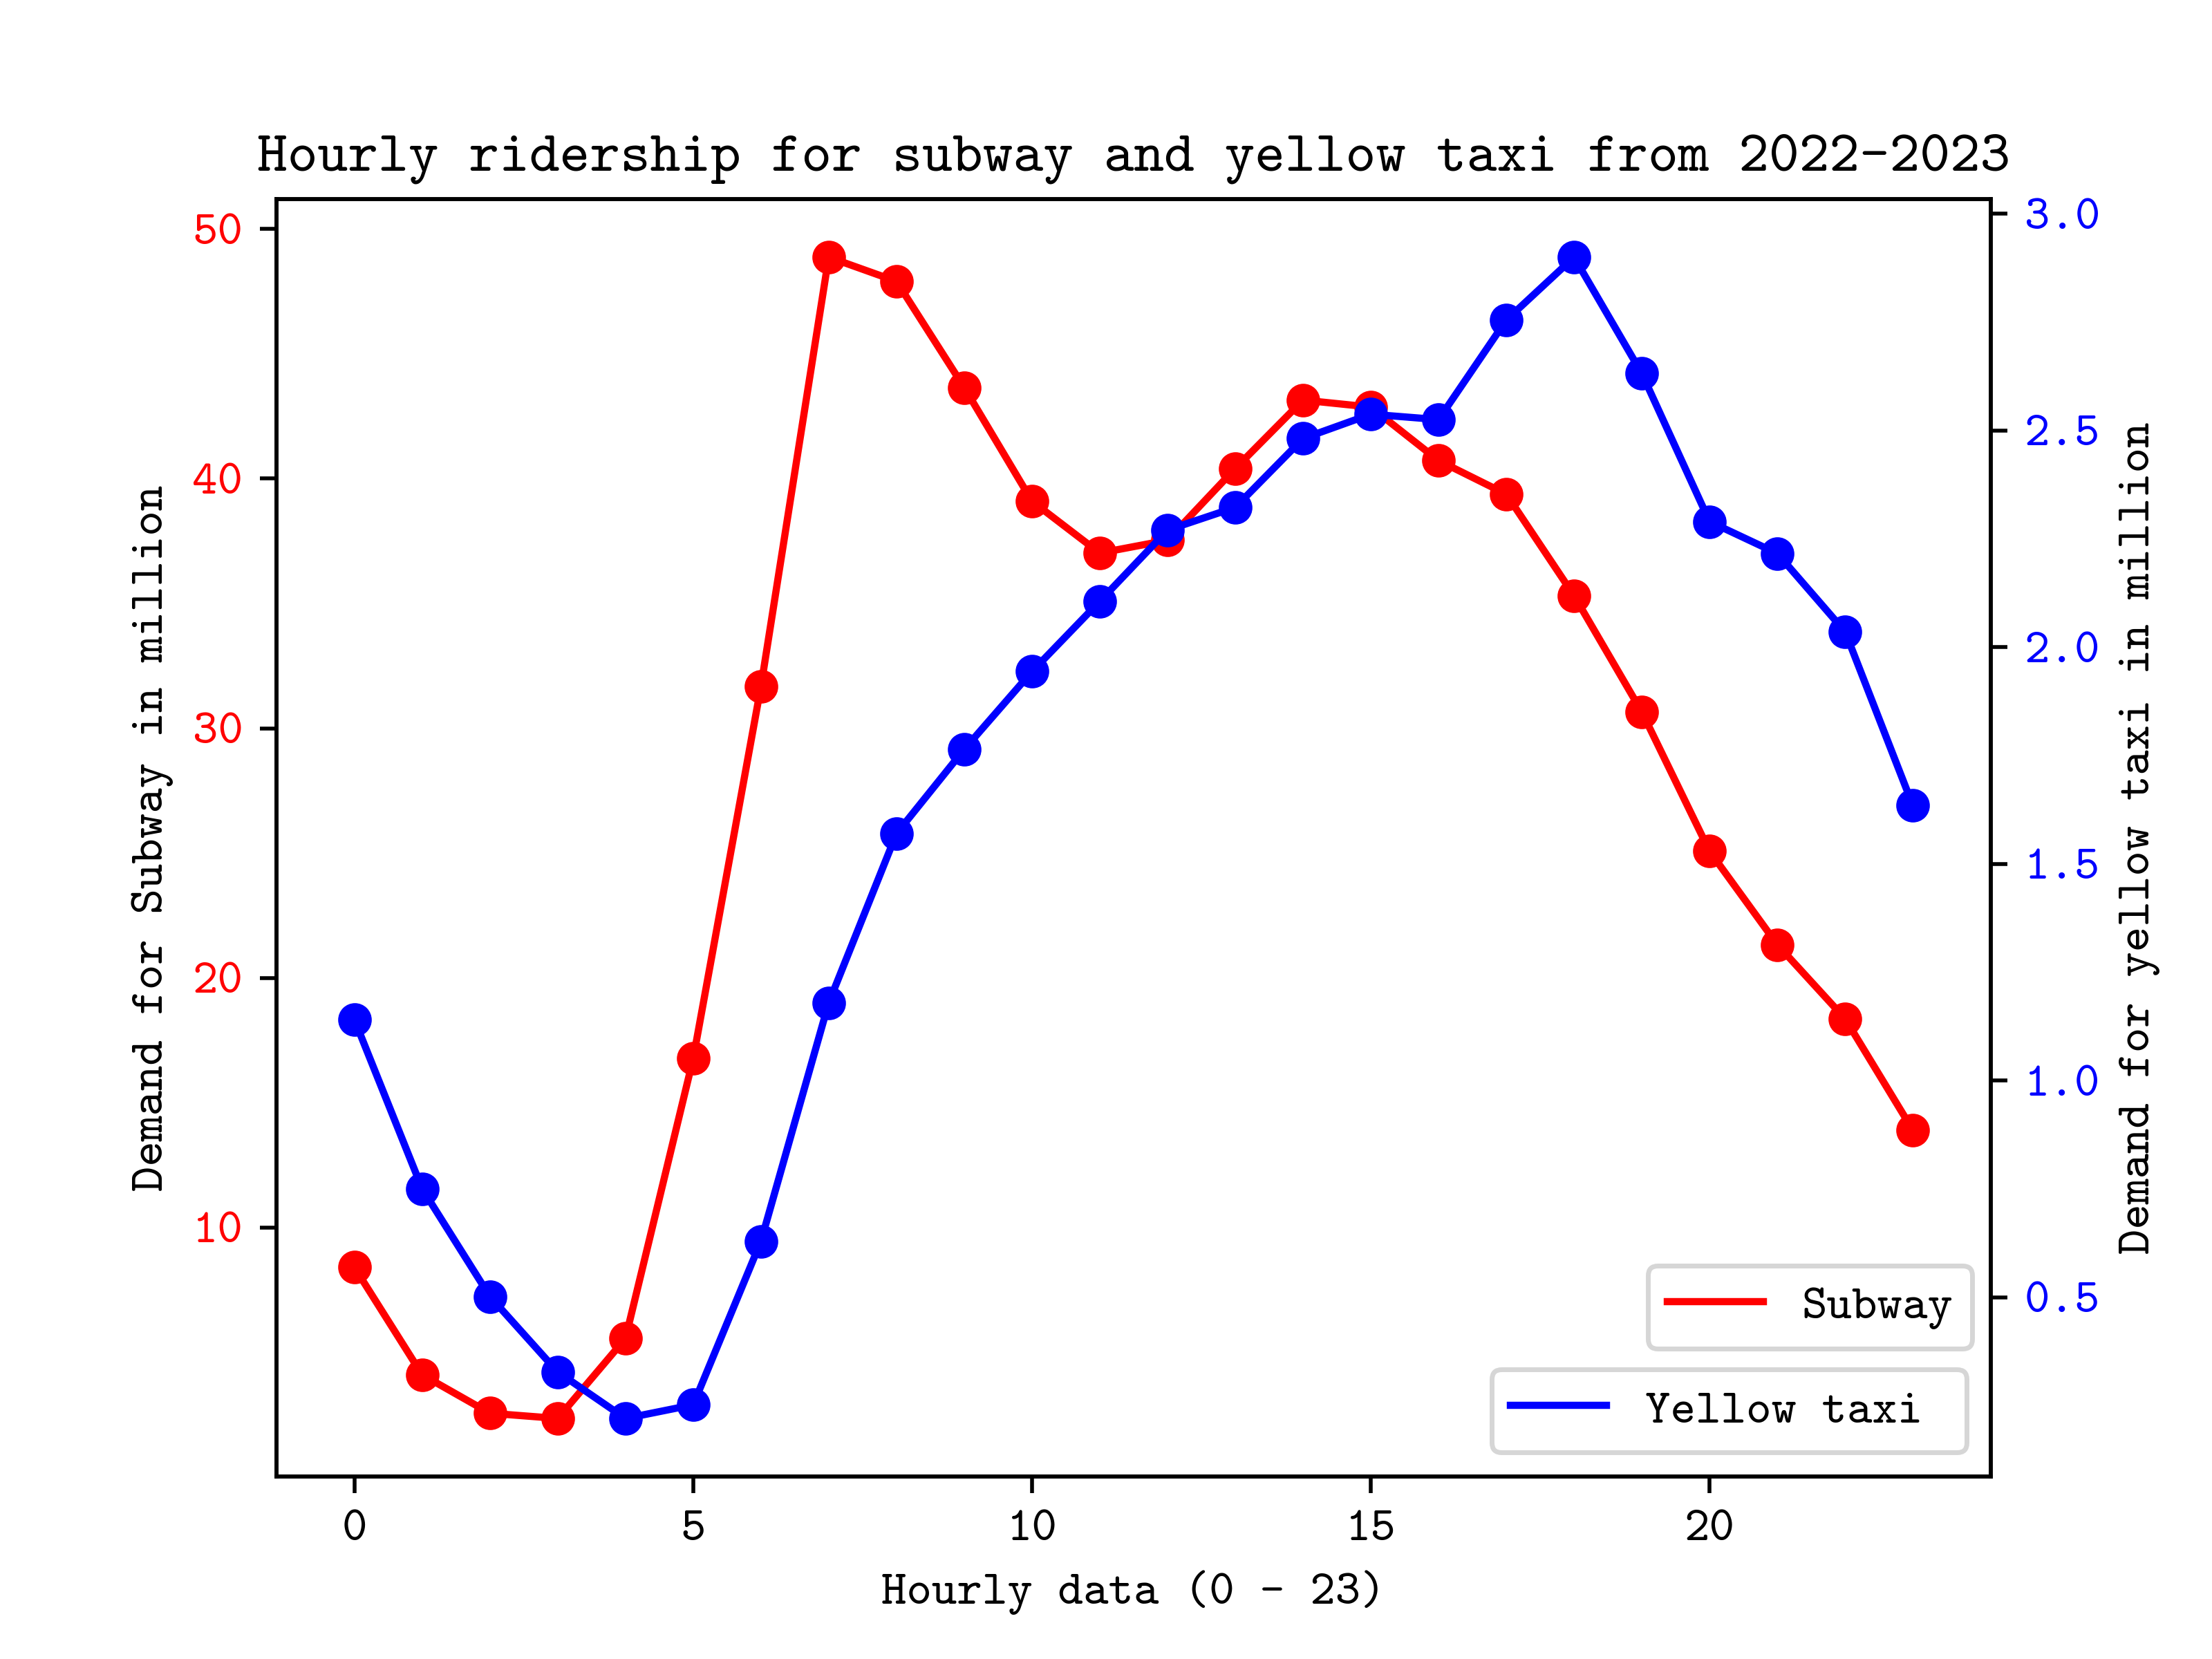
\includegraphics[width=\textwidth]{plots/yellow_subway.png}
        \caption{Hourly ridership for subway and yellow taxi}
        \label{subfig:mta_taxi}
    \end{subfigure}
    \hfill
    \begin{subfigure}[b]{0.45\textwidth}
        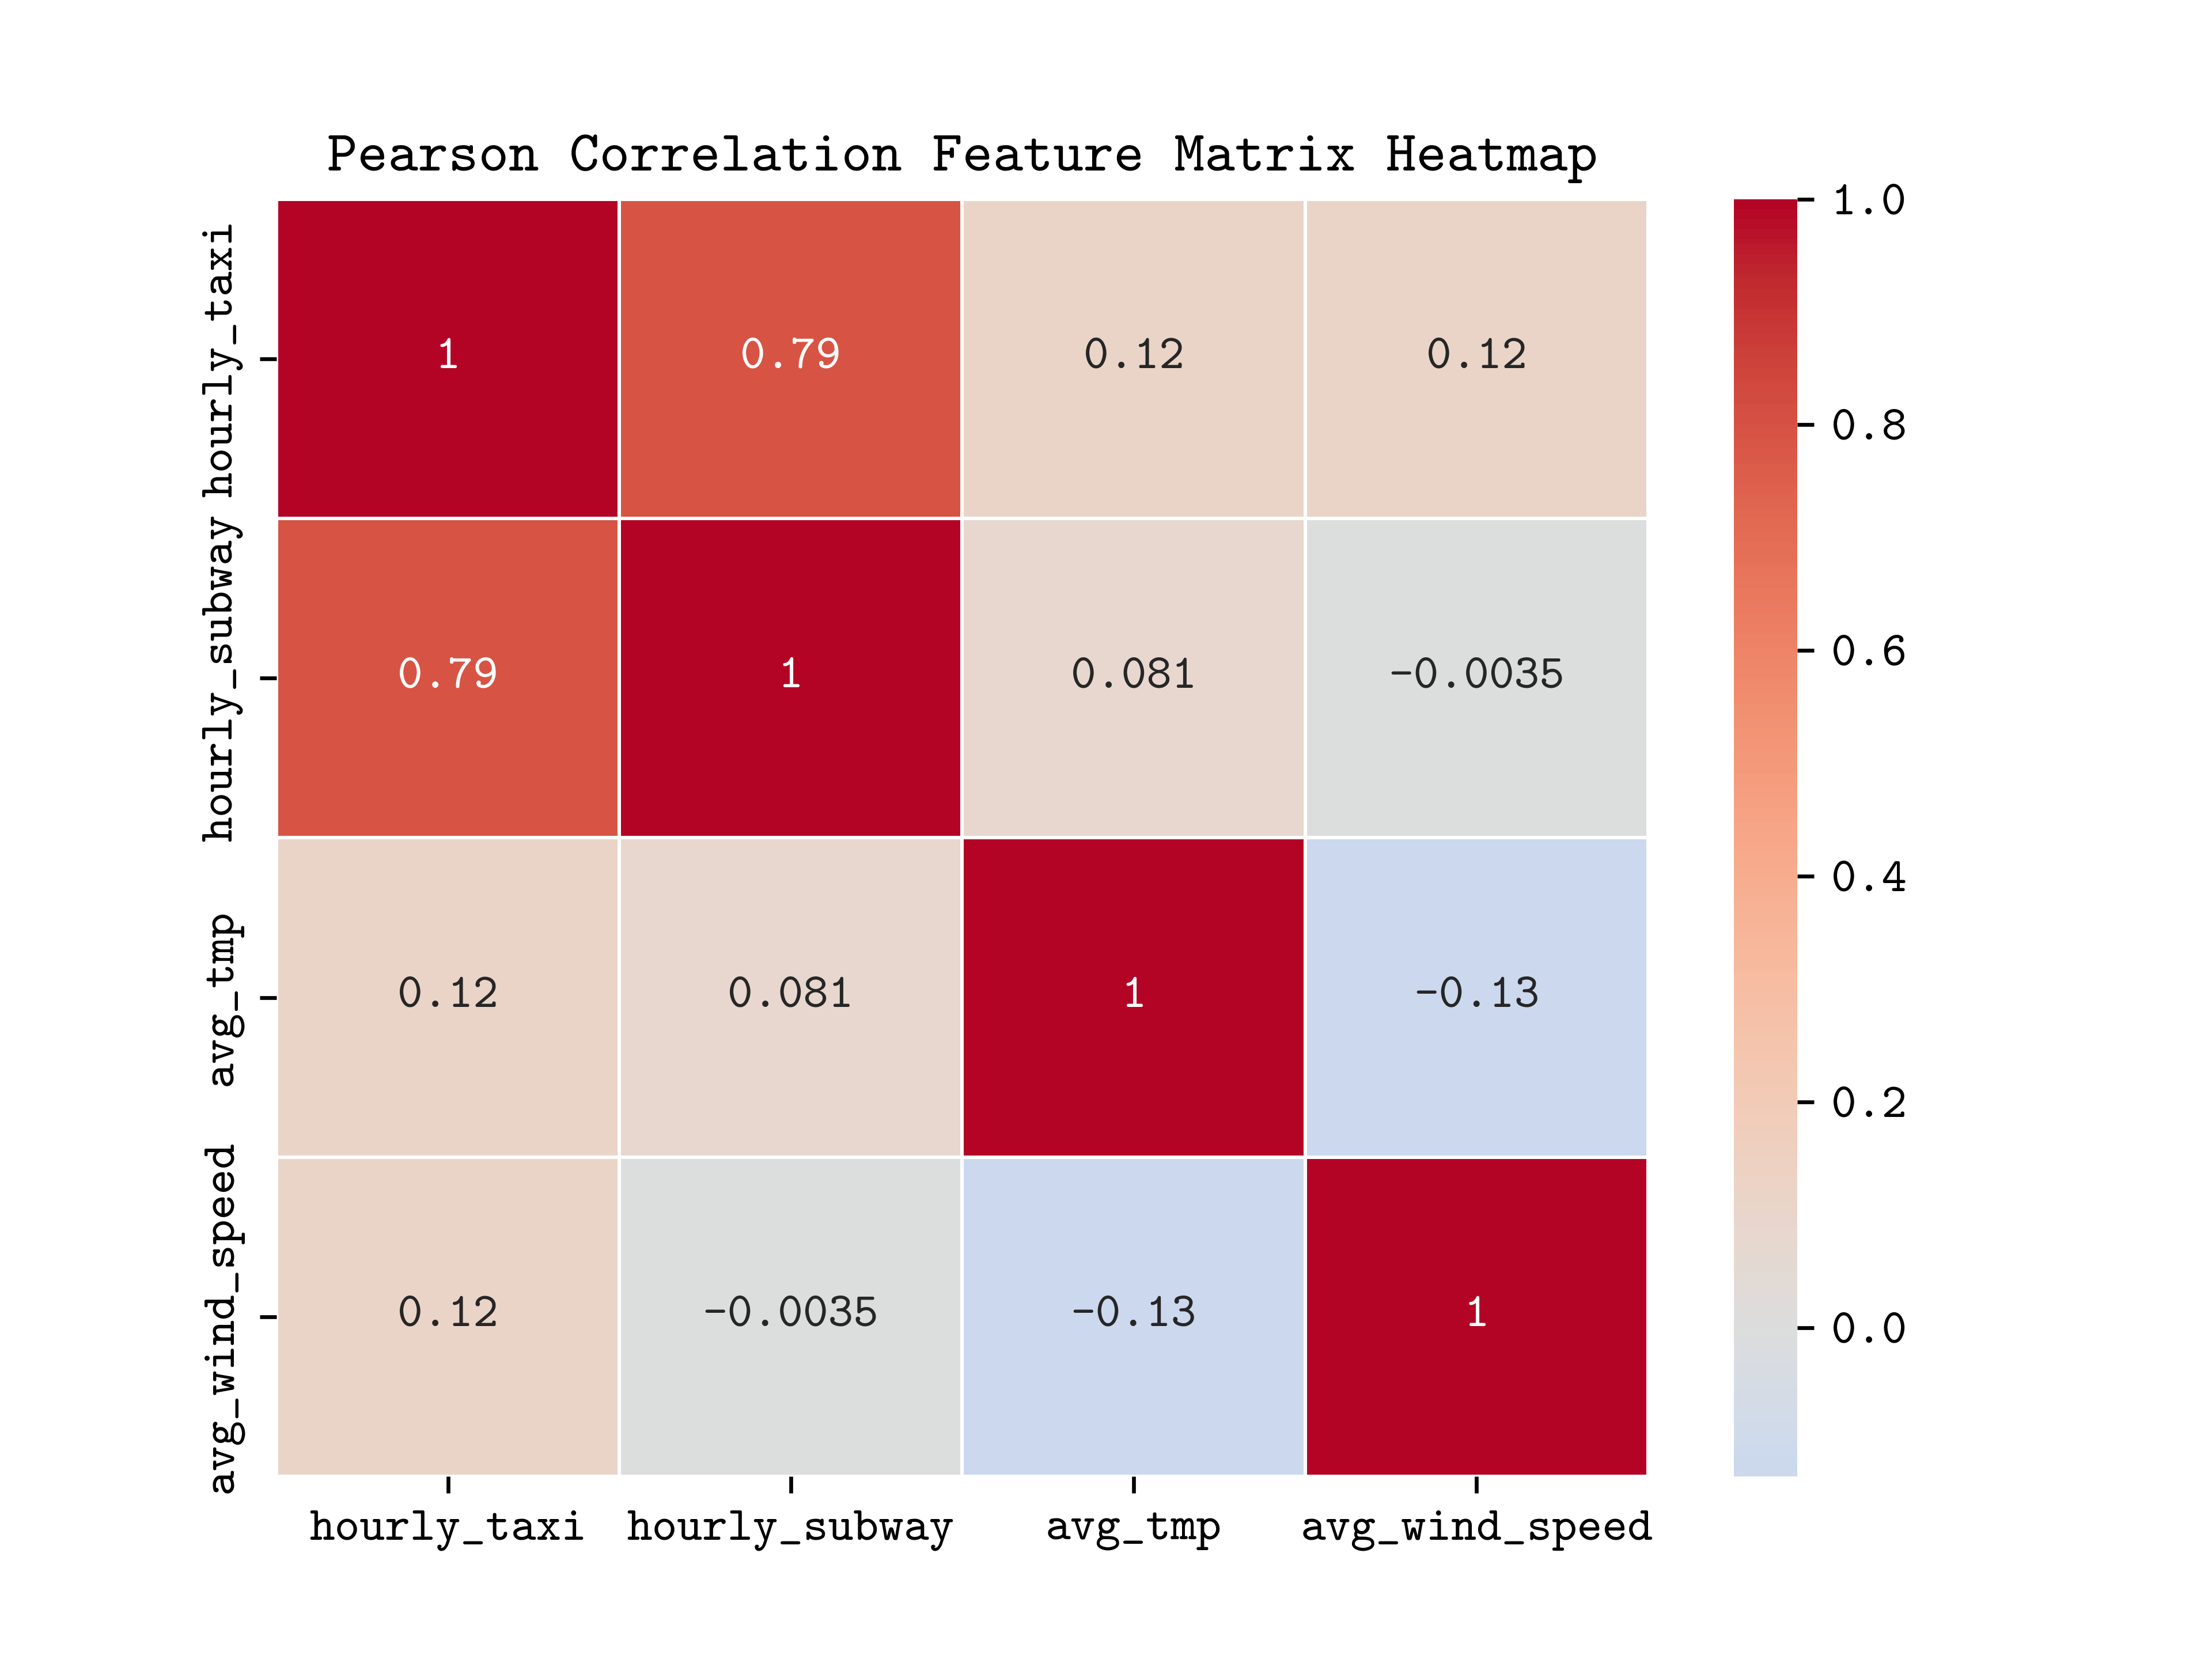
\includegraphics[width=\textwidth]{plots/pearson_correlation.png}
        \caption{Pearson Correlation for Manhattan borough }
        \label{subfig:plot2}
    \end{subfigure}
    \caption{Feature analysis for weather and subway features}
    \label{fig:pearson correlation}
\end{figure}

Despite low correlation between \texttt{temperature}, \texttt{wind\_speed} and response variable \texttt{count}, these features are retained during feature selection. Real-world cases as illustrated by Tan(2022) and Pfosi(2022), showcased that during extreme weather events, the demand for cab was substantially reduced, signalling weather variables are highly powerful for modelling \cite{Ming, NickPfosi}.

Regarding \textbf{feature distribution}, while the boxplots for \texttt{Hourly taxi ridership} and \texttt{Hourly subway ridership} exhibit left-skewness, that for hourly temperature is a relatively right-skewed distribution, within a reasonable range from -15 to 35 degrees Celcius. The box plot also reveals outliers in hourly wind speed, with speed exceeding 12.5 meters/second. The author decides not to remove these outliers as they have passed all quality control checks from NCEI data source with quality code of 5. Given the city's unusual weather events such as storms, these outliers are considered reasonable.  

\begin{figure}[ht]
    \centering
    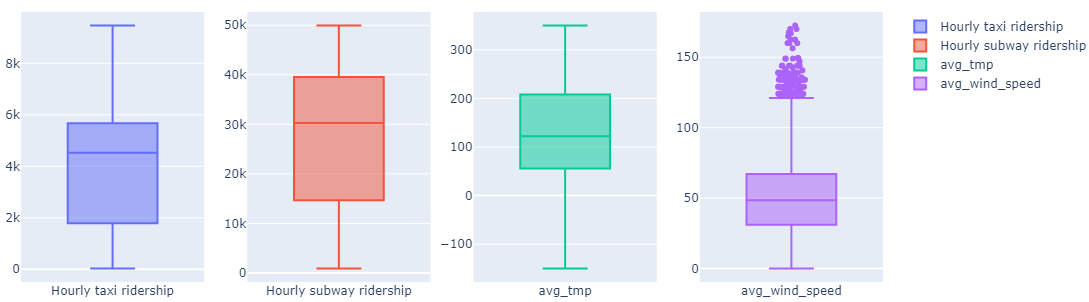
\includegraphics[width=1.0\textwidth]{plots/boxplot2.jpg}
    \caption{Feature Distribution Boxplots}
    \label{fig:feature distribution}
\end{figure}
Regarding missing data for modelling, only 1 out of 9432 instances is found missing in Manhattan borough, which is 0.01\% of the dataset. Therefore, linear interpolation based on preceding and subsequent timestamps is implemented for imputation \cite{Pandas-Interpolate}. 

\section{Modelling, an end-to-end example with Manhattan}
As mentioned in Section 3, this study will exclusively conduct modelling in Manhattan, the busiest borough where yellow taxi has an unique advantage. Manhattan data (9432 instances, 5 features) is transformed via window sliding method \cite{Tran-NBeats}, involving iterative traversal and collection of time-series features and their corresponding responses.


\subsection{Methodology overview}
  Based on a time series \begin{math}\{\boldsymbol{x_{1}}, \boldsymbol{x_{2}},..., \boldsymbol{x_{w}}\}\end{math} where $\boldsymbol{x_{i}}$ is a vector of $n$ features at time $i$, a time series forecasting algorithm needs to learn the input and returns a function that maps input to predicted values for response variable $y$ from time $w + 1$ to $w+k$ for some pre-chosen $k\ge1$. For example, for $w$ is 96, and $k$ is 4, which means based on data from the previous 96 hours, we are going to predict yellow taxi demand in the next 4 hours.
\begin{equation}
    {y}_{w+i} = f_{i}(\boldsymbol{x_{1}},\boldsymbol{x_{2}},...,\boldsymbol{x_{w}}) + \epsilon_{i} \    \text{for} \    1\leq i \leq k\end{equation}

where ${y}_{w+i}$ is the response variable value for time $w+i$, $w$ is the window size, $k$ is the future length we need to predict, $f_{i}$ is the prediction function at time $w+i$ learned from data by deep learning methods, and $\epsilon_{i}$ is the random error - $\epsilon_{i} \sim \mathcal{N}(0,\,\sigma^{2})$. 

The dataset is then partitioned approximately in ratio: 70\% for training (February 2022 - October 2022), 15\% for validation (November 2022 - December 2022), and 15\% for testing (January 2023 - February 2023)

\begin{figure}[ht]
    \begin{minipage}{0.6\linewidth}
        \begin{adjustbox}{left}
            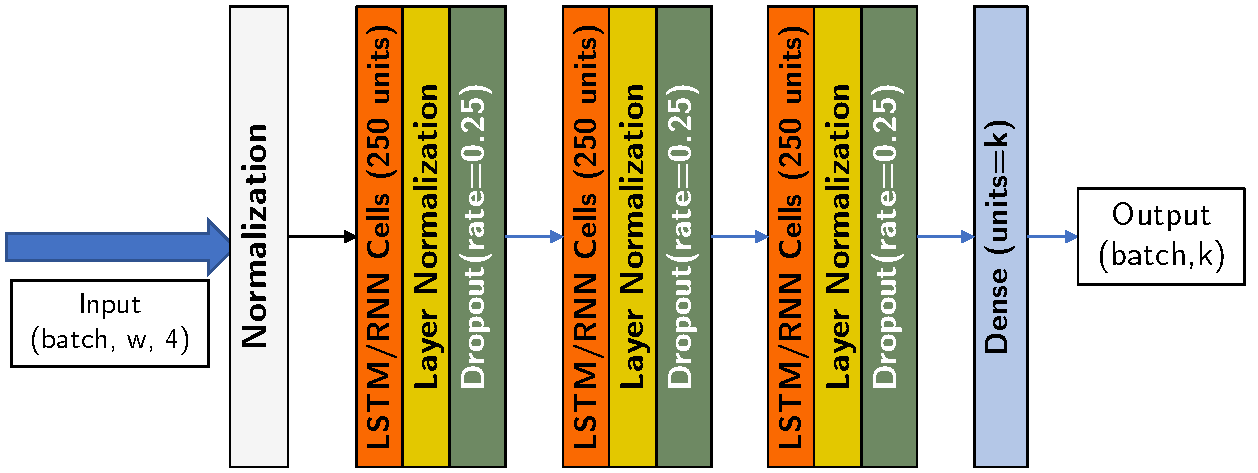
\includegraphics[width=\textwidth]{plots/architecture.pdf}
            
        \end{adjustbox}
    \end{minipage}
    \begin{minipage}{0.4\linewidth}
       The data is then fed into 2 Deep Learning Networks, as illustrated in the left. The network utilizes Seq2Seq approach, implementing LSTM (Long Short-Term Memory) or GRU (Gated Recurrent Units) as its components layers. Both LSTM and GRU are known for their exceptional capabilities to process sequential data, thanks to their brilliant architecture using gates \cite{Sak-LSTM, Chung-GRU}.  
    \end{minipage}
        \caption{Deep Learning Architectures}
    
    \label{fig:architecture}
\end{figure}

\section{Error analysis}

For this experiment, we will be examining both deep learning architectures in various prediction steps (different future steps) based on training loss of \textbf{Mean Squared Error}, and evaluation metrics of \textbf{RMSE} . The overall results are summarized in the table below:  

\begin{figure}[ht]
    \begin{minipage}{0.45\textwidth}
        \centering
        \begin{tabular}{|l|c|c|}
            \hline
            Future prediction (k) & LSTM & GRU \\
            \hline
            1 hour & 750.02 & \textbf{686.46} \\
            4 hours & 934.55 & \textbf{776.28} \\
            16 hours & 991.13 & \textbf{924.81} \\
            \hline
        \end{tabular}
        \caption{Performance (RMSE) at \\ various k for w = 96}
        \label{table:prediction}
    \end{minipage}%
    \begin{minipage}{0.45\textwidth}
        \centering
        \begin{tabular}{|l|c|c|}
            \hline
            Window size (w) & LSTM & GRU \\
            \hline
            1 day & 954.09 & \textbf{871.37} \\
            2 days & 936.43 & \textbf{922.47} \\
            8 days & \textbf{950.24} & 986.12 \\
            \hline
        \end{tabular}
        \caption{Performance (RMSE) at various w for k = 8}
        \label{table:window}
    \end{minipage}
\end{figure}



Overall, among the 2 models, GRU networks outperforms LSTM in terms of model's performance (smaller error bolded) because GRU tends to be more powerful than LSTM in small datasets \cite{Chung-GRU}. More importantly, as the future prediction steps in Table \ref{table:prediction} increase, the errors observed in both models also increase, which is consistent with the intuition that the more uncertain about the future, the greater error models are likely to make \cite{Tran-NBeats}.


Another key conclusion from Table \ref{table:window} is that the greater the window size w, the worse performance GRU network attains, which is reasoned by conditional on more recent data, the response variable and older predictors are weakly related. Therefore, using a large window size w will introduce a higher dimension of covariates with few useful information, resulting in a decline in model's performances \cite{Tran-NBeats}. 
% However, LSTM's performance slightly improves with two-day window before declining as window size reaches 8 days, which follows previous conclusion. This behavior stems from LSTM's superior capability in capturing  the long-range high-complexity sequences compared to GRU, making it the better model for large window size. 

However, when the look-back window is large, LSTM becomes the more powerful model, which is explained by LSTM's superior capability in capturing  the long-range high-complexity sequences. Therefore, depending on different purposes whether long or short forecasting for instance, TLC should be cautious in their choice of model and other hyperparameters for the best of their interests.

% Dropout Layers, LayerNormalization, and Early Stopping are embedded into the architecture of both models to prevent overfiting in Figure \ref{fig:architecture}. From Figure \ref{fig:geospatial time}, it was not until the 17\^{th} and 15\^{th} epochs that LSTM and GRU models started to over-fit respectively, and the training process was then terminated to avoid overfit. Additionally, the validation loss curve from GRU model is also smoother and terminated longer than LSTM model, signalling a better model for single step prediction.



% \begin{figure}[ht]
%     \centering
%     \begin{subfigure}[b]{0.45\textwidth}
%         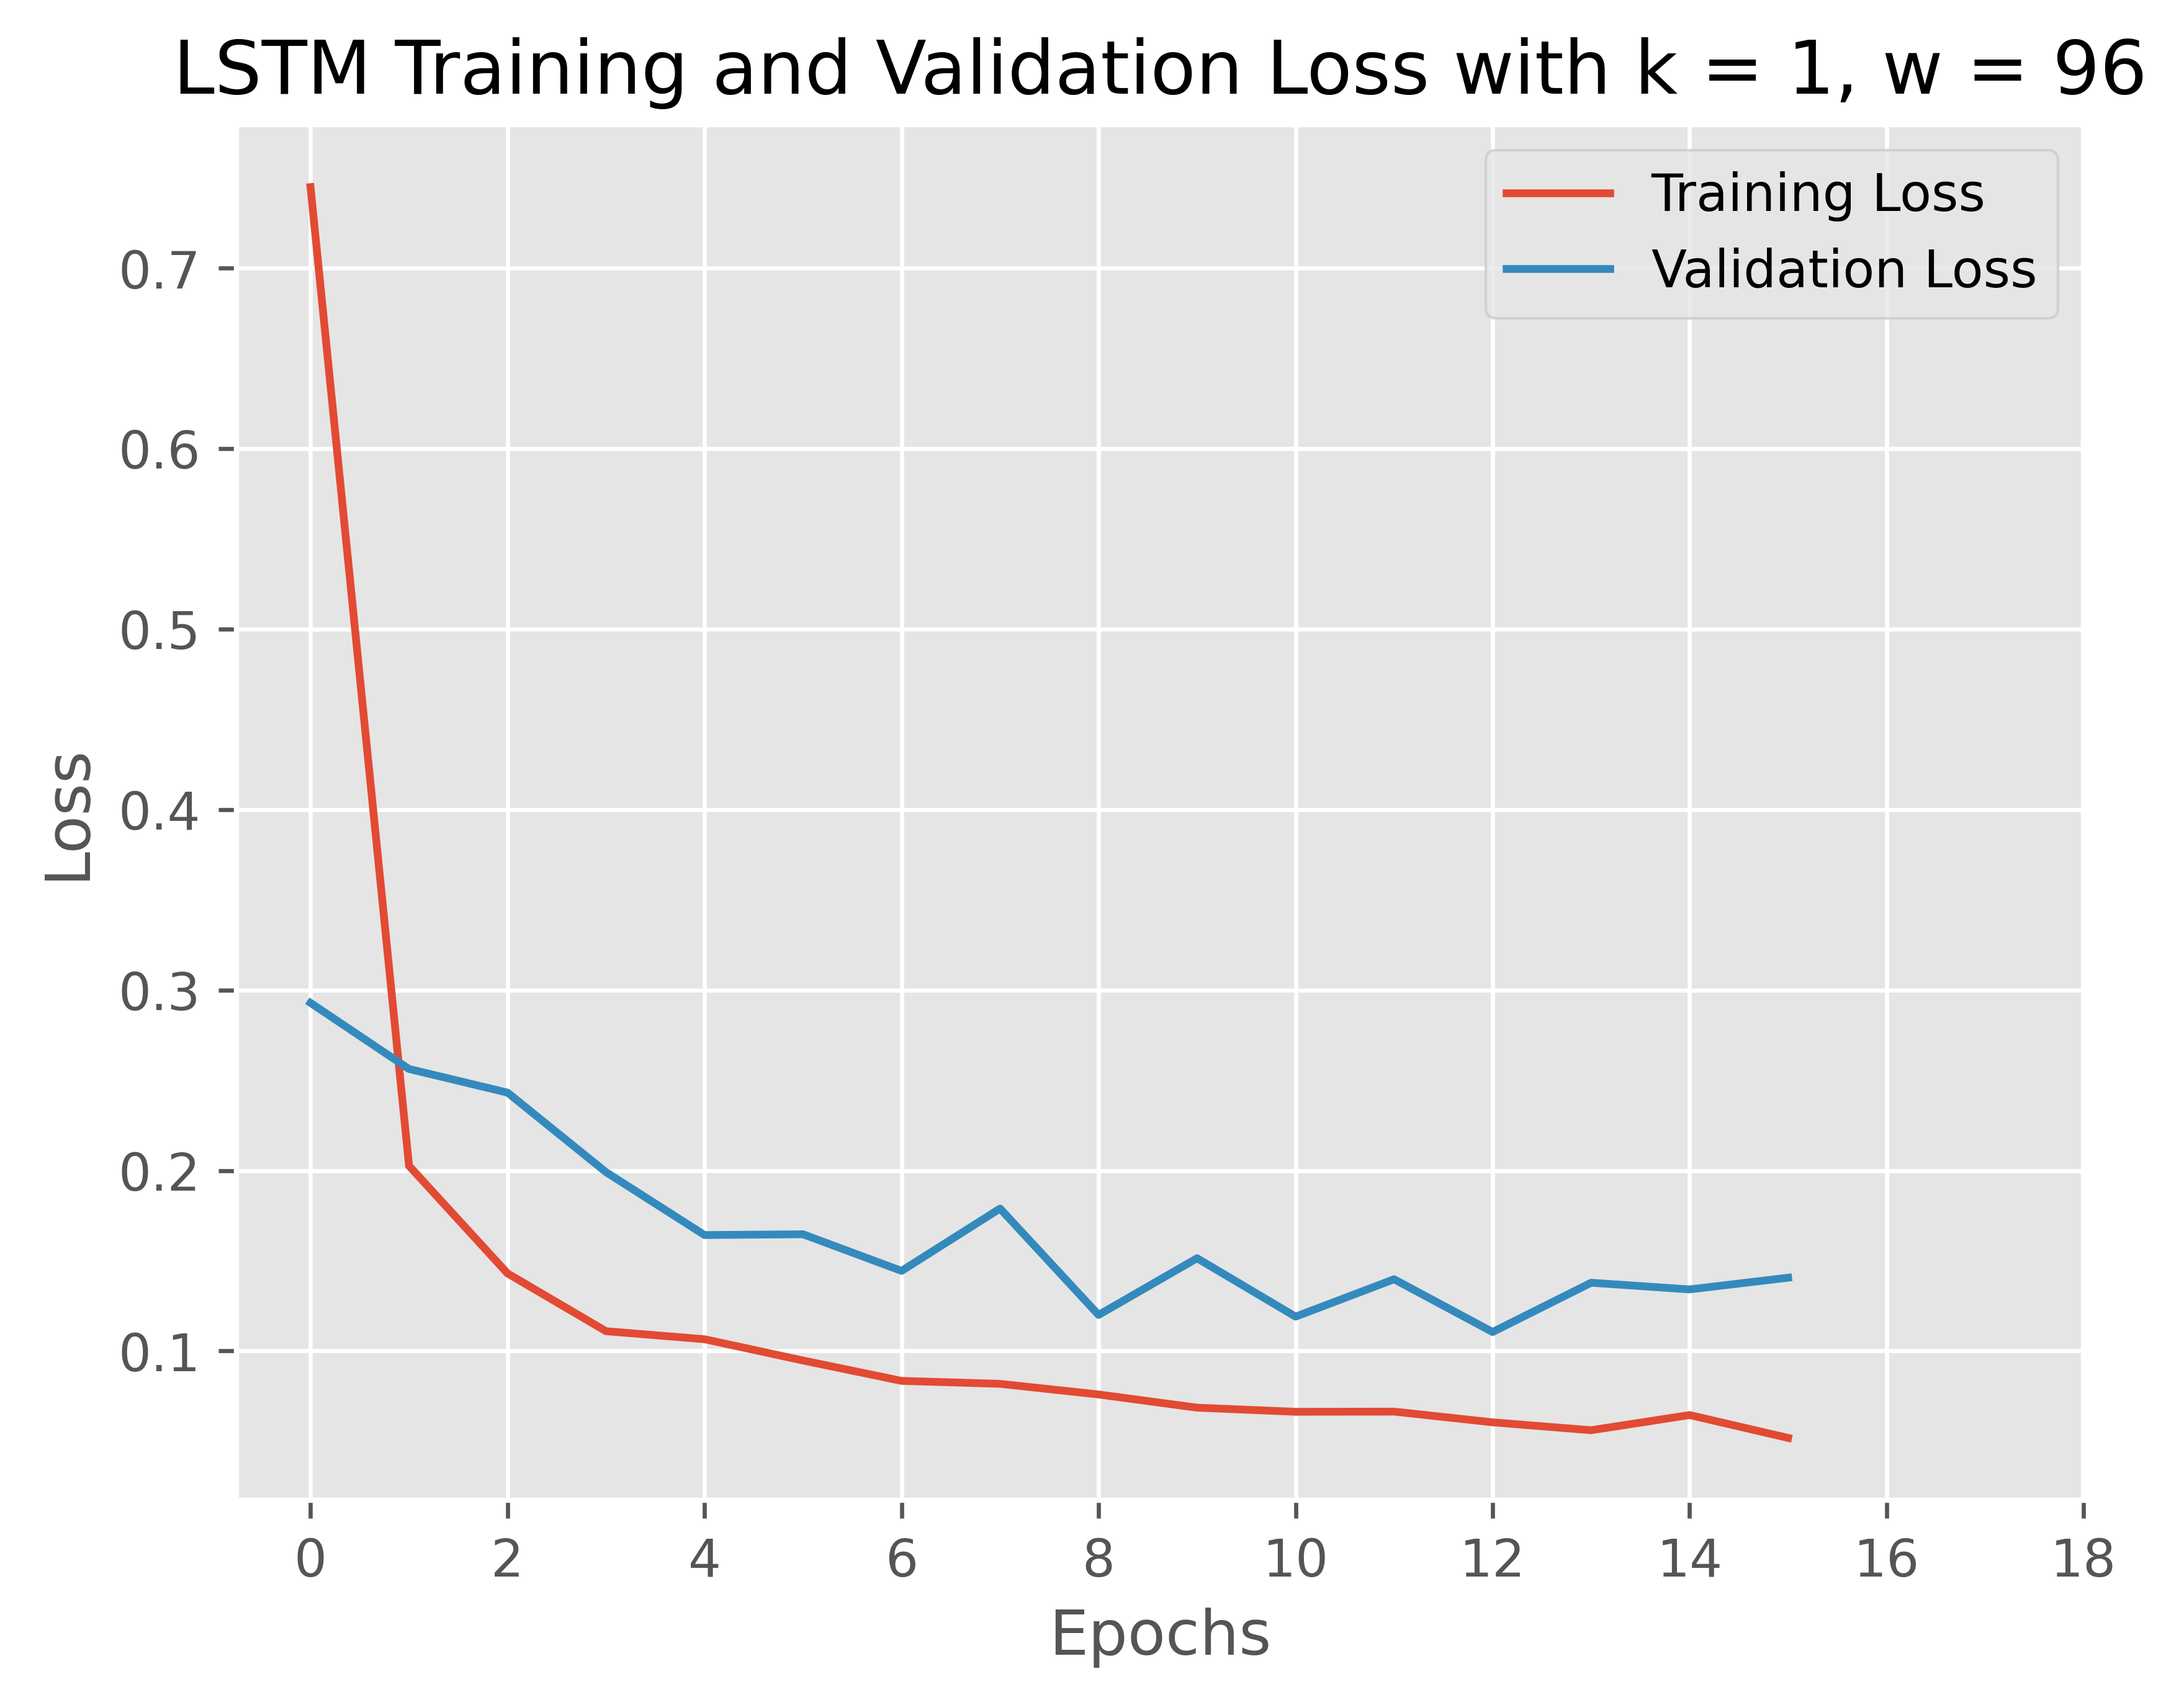
\includegraphics[width=\textwidth]{plots/LSTM.png}
%     \end{subfigure}
%     \hfill
%     \begin{subfigure}[b]{0.45\textwidth}
%         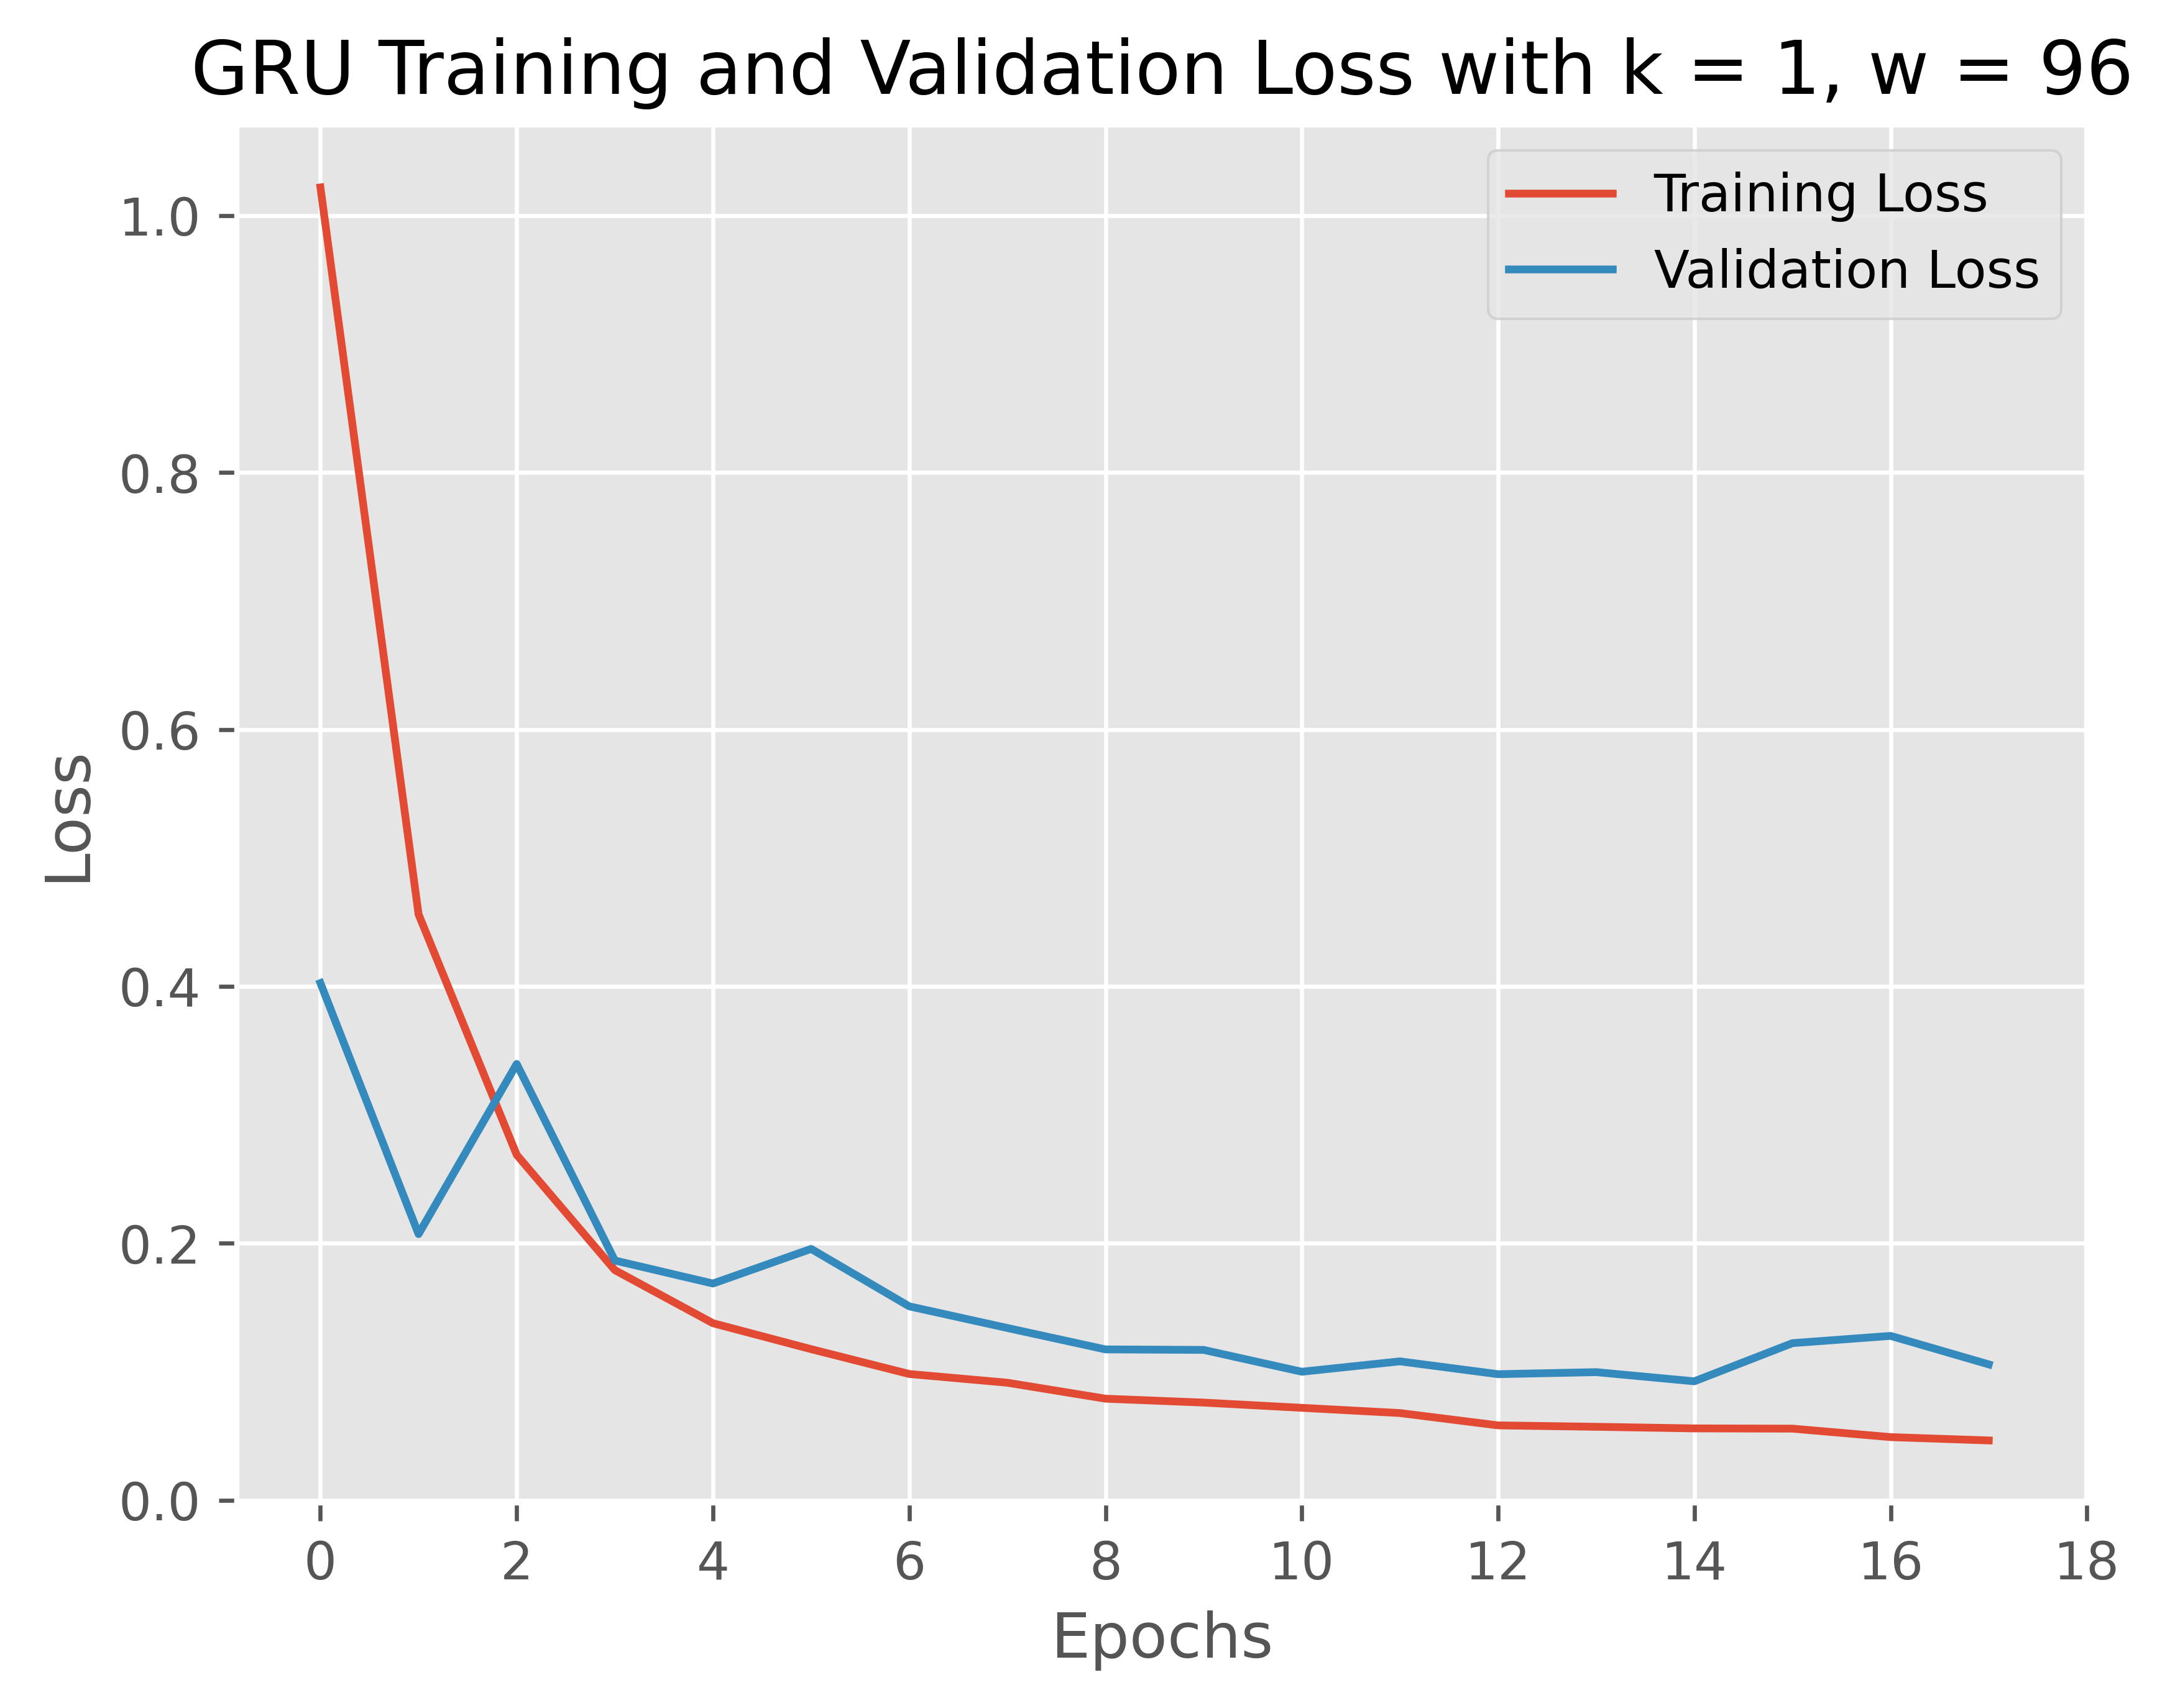
\includegraphics[width=\textwidth]{plots/GRU.png}
%     \end{subfigure}
%     \caption{Training and validation loss curve for 2 models (k = 1, w =4)}
%     \label{fig:validation curve}
% \end{figure}

\begin{figure}[ht]
    \centering
    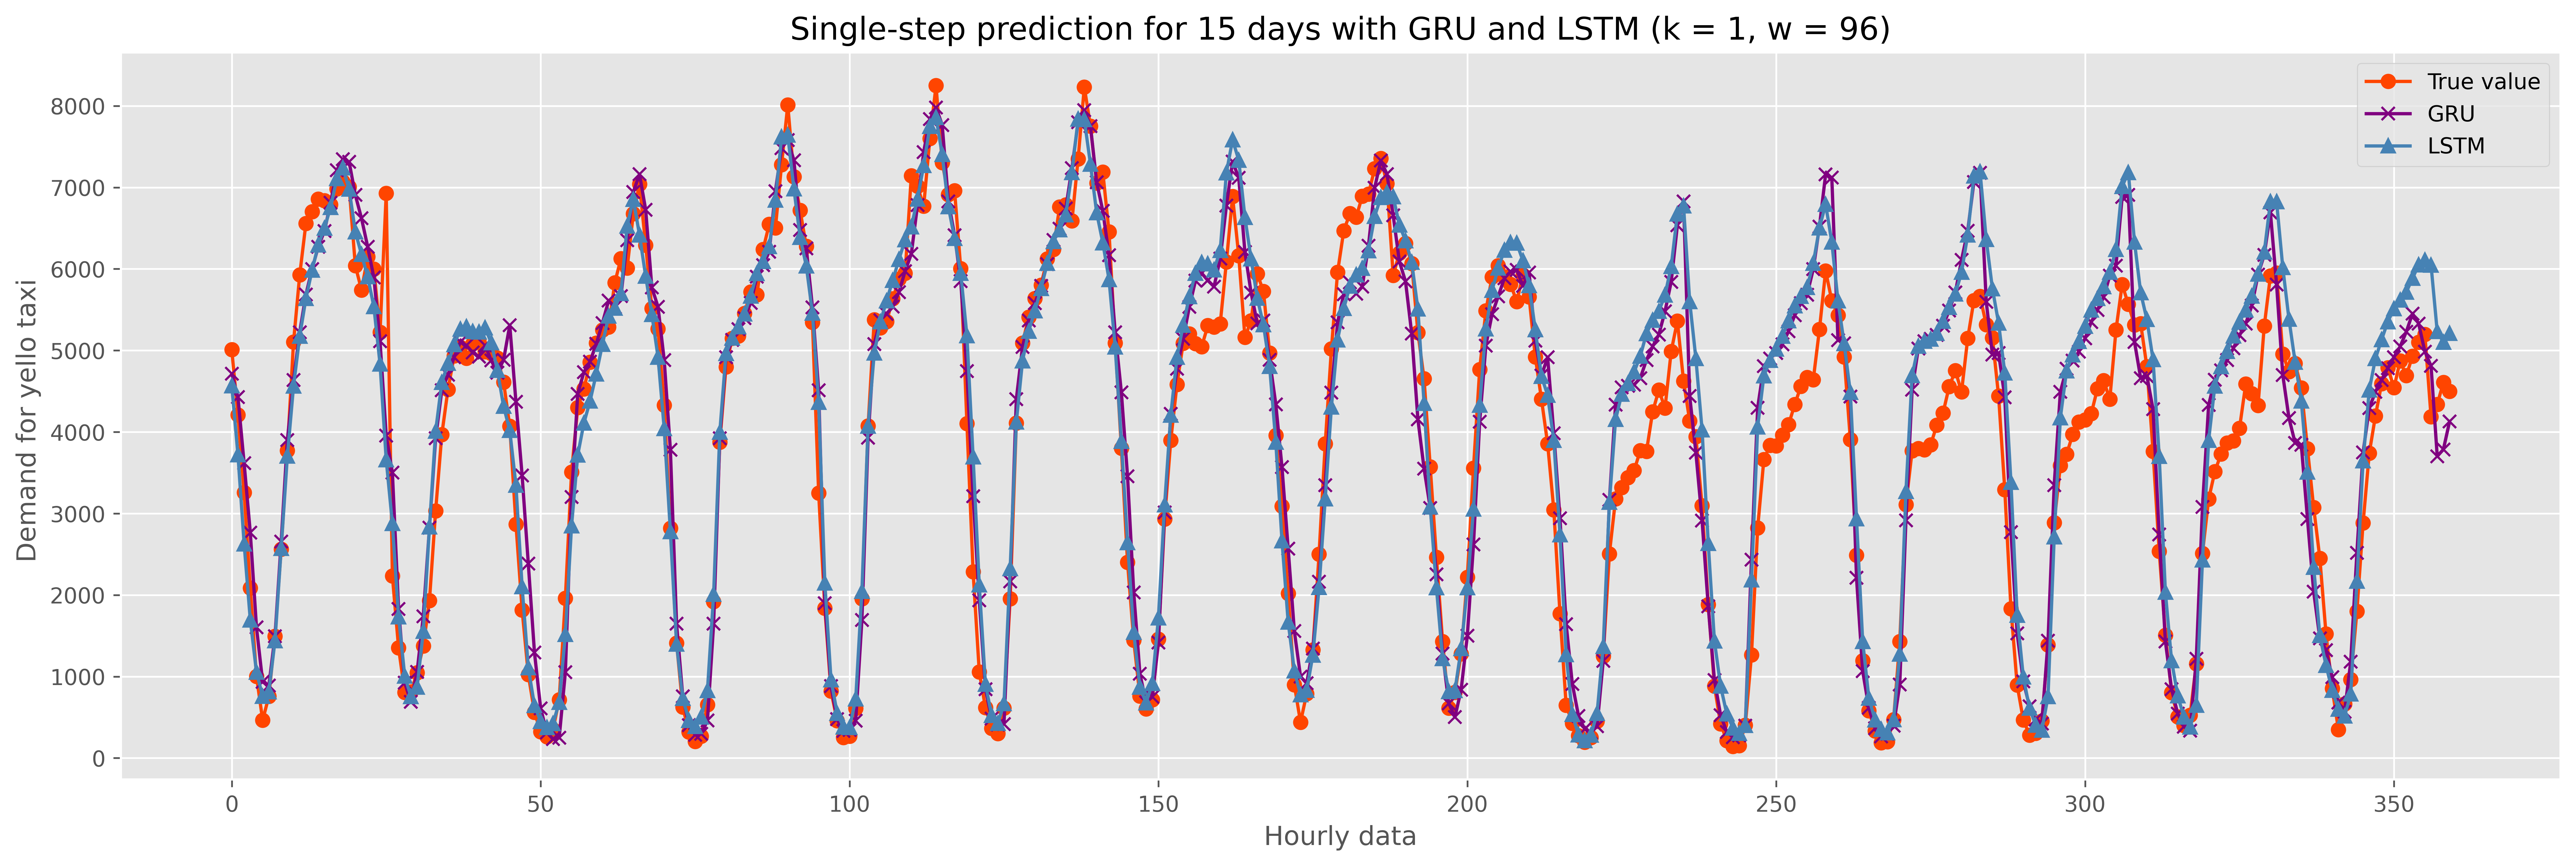
\includegraphics[width=0.8\textwidth]{plots/better.png}
    \caption{Single-step prediction for 15 days with GRU and LSTM (k=1, w=96)}
    \label{fig:singlestep}
\end{figure}

Figure \ref{fig:singlestep} shows both architectures have achieved strong performance when the predicted values closely match the ground truth; however, GRU is the more powerful model, as illustrated in Table \ref{table:prediction} and Table \ref{table:window}. In addition, the highest demand for yellow taxi is during the noon when there is a peak during this period every 24 hours, which implies that TLC should encourage their yellow taxi drivers to be around Manhattan due to peak demands.  

However, from 150\textsuperscript{th} hour (January 6, 2023), both models over-estimated the true demand, which could be several factors including seasonal factor, which could be improved by introducing a complex seasonal decomposition block to account for the seasonal factor. However, the models' performance are strong enough illustrated by competitve results and errors.


\section{Recommendations}
Figure \ref{fig:geospatial time}b suggests that during daytime hours, TLC should suggest yellow taxi drivers target at high-demanded areas such as JFK, Laguardia Airport and Manhattan. However during the nights and early morning, only JFK and a region of Manhattan should be targeted. Highly-demanded regions comprise of a variety of entertainment establishments such as restaurants and night clubs. Therefore, within Manhattan, TLC should propose taxi drivers with some regions namely Diamond District) illustrated in Figure \ref{fig:potential market}, hosting numerous clubs and bars; which is the potential market as intoxicated customers usually opt for a private means of transport.

\begin{figure}[ht]
    \centering
    \begin{subfigure}[b]{0.4\textwidth}
        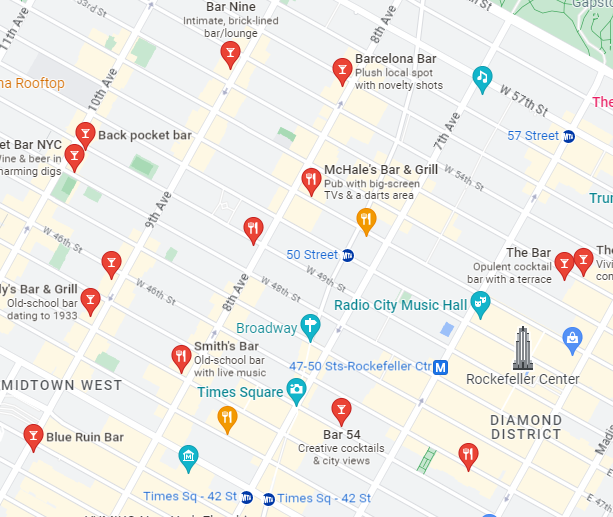
\includegraphics[width=\textwidth]{plots/diamond.png}
        \caption{Diamond District - potential market during the nights}
        \label{fig:potential market}
    \end{subfigure}
    \hfill
    \begin{subfigure}[b]{0.3\textwidth}
    \centering
        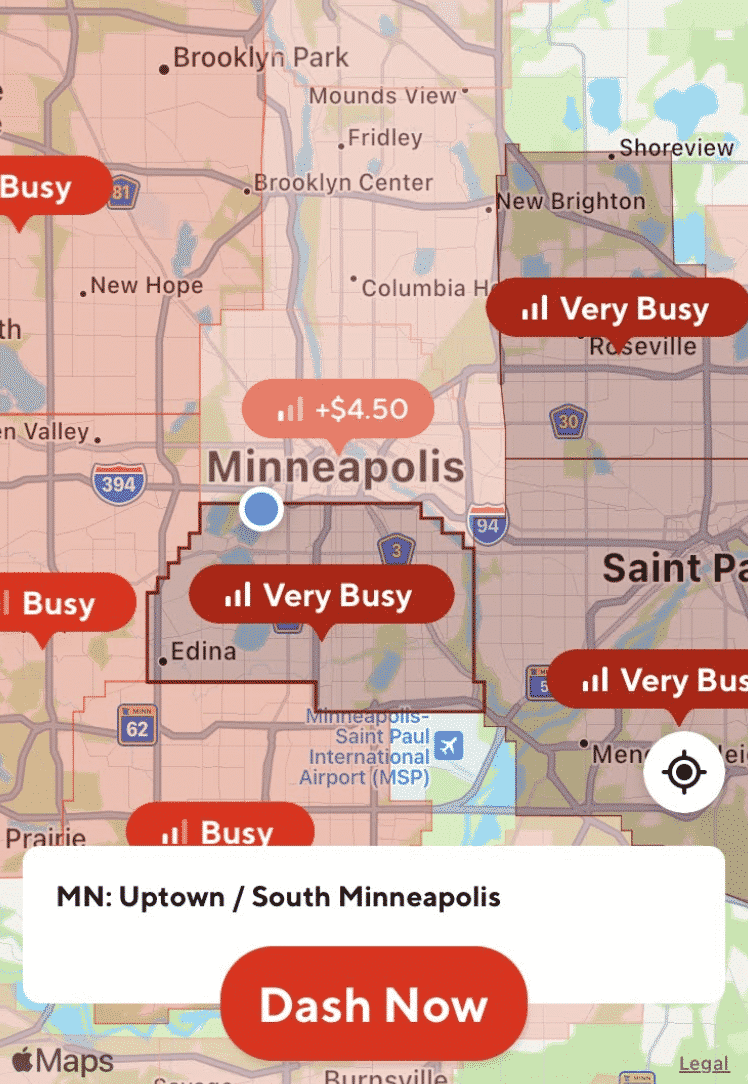
\includegraphics[width=\textwidth]{plots/financial partner.png}
        \caption{DoorDash App - an example interface navigating their shippers towards busy zones}
        \label{subfig:plot2}
    \end{subfigure}
    \caption{Recommendations for TLC}
    \label{fig:doordash}
\end{figure}

Figure \ref{fig:singlestep} has illustrated how precise both models could be although they are foundational and basic. Hence, TLC should consider investing towards hiring machine learning engineers to apply transfer learning on SOTA pretrained models such as Temporal Fusion Transformer and Autoformers or design a novel architecture. Given data is the core element of deep learning,  their competitive advantage in terms of massive data collection facilitates generating highly accurate predictions.\\
    
With a highly powerful model in hand, TLC could conduct training process at a smaller scale based on zone location ID Madison Square for instance, instead of the entire borough. Building an app accessing these crucial model predictions will act as a reference/assistant to help yellow taxi drivers understand about substantially-demanded zones, from which they could approach. This plan is certainly achievable as a similar case DoorDash, a food shipping business, has already developed an app to help their shippers earn money more efficiently as in Figure \ref{subfig:plot2}. 

% \begin{figure}[ht]
%     \begin{minipage}{0.6\linewidth}
% Figure \ref{fig:geospatial time}b suggests that during daytime hours, TLC should suggest yellow taxi drivers target at high-demanded areas such as JFK, Laguardia Airport and Manhattan. However during the nights and early morning, only JFK and a region of Manhattan should be targeted. Further analysis found that this particular crowded region comprises of a variety of entertainment establishments such as restaurants and night clubs. Therefore, within Manhattan, instead of aimlessly targeting at Financial District and surrounding areas, TLC should propose taxi drivers with some regions namely Diamond District (included in the hot zone), hosting numerous clubs and bars; which is the potential market as intoxicated customers usually opt for a private yet safe means of transport to retreat.

%     \end{minipage}
%     \begin{minipage}{0.4\linewidth}

%       \begin{adjustbox}{right}
%             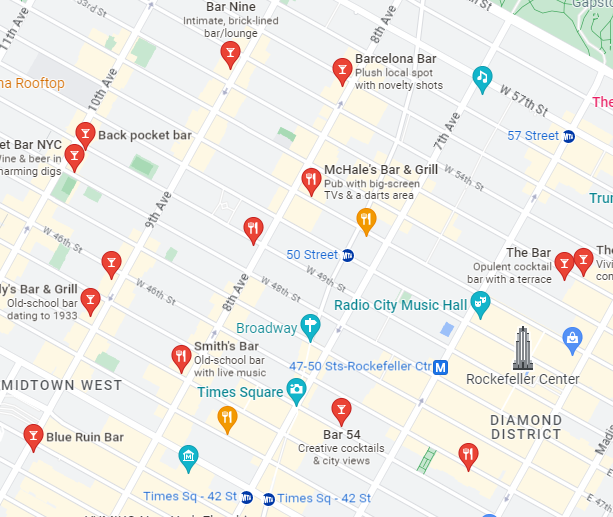
\includegraphics[width=\textwidth]{plots/diamond.png}
            
%         \end{adjustbox}
%     \end{minipage}
%         \caption{Potential market for yellow taxi drivers}
    
%     \label{fig:potential market}
% \end{figure}






% \begin{figure}[ht]
%     \begin{minipage}{0.4\linewidth}
%         \begin{adjustbox}{left}
%             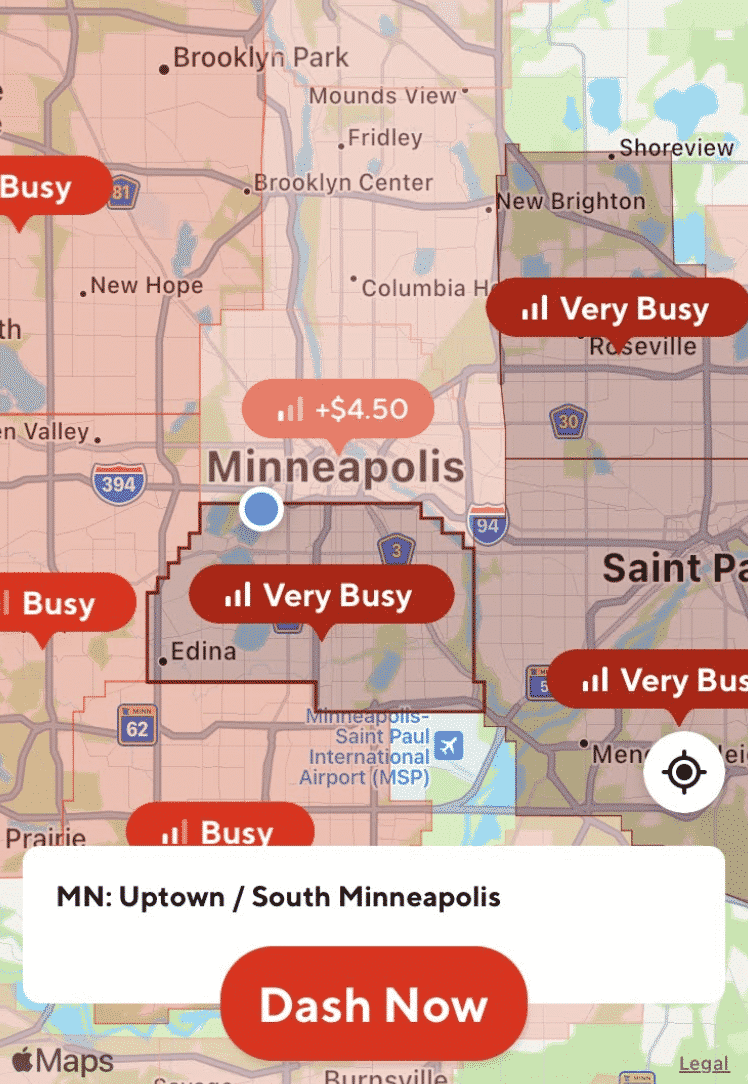
\includegraphics[width=\textwidth]{plots/financial partner.png}
            
%         \end{adjustbox}
%     \end{minipage}
%     \begin{minipage}{0.6\linewidth}
%     Figure 9 has illustrated how precise both models could be although they are foundational and basic. Current state-of-the-art transformer-based models and variants such as Temporal Fusion Transformer and Autoformer have achieved highly competitive results. Hence, TLC should consider investing towards hiring machine learning engineers to apply transfer learning on pretrained models or design a novel architecture. Given data is the core element of deep learning,  their competitive advantage in terms of massive data collection facilitate
%     s generating highly accurate predictions.\\
    
% In the future, TLC should implement this model in a smaller scale based on zone location ID, Madison Square for instance. Building an app with this interface adopted from DoorDash (food shipping business) will act as a reference to help yellow taxi drivers understand about substantially-demanded zones, from which they could target. 
%     \end{minipage}
%         \caption{DoorDash App - an example interface navigating their shippers towards busy zones}
    
%     \label{fig:leftalignedplot}
% \end{figure}


\section{Conclusion}
This research focuses on a real-world application of time series forecasting on the demand for yellow taxi in inner urban areas of New York City, with an end-to-end example on Manhattan. With the help integration of external datasets such as Hourly Integrated Surface Database and MTA Subway Dataset, this has created a simple yet highly effective in forecasting the demand.

Different experiments with various hyper-parameters have been conducted to help TLC understand about the models output and its potential. Therefore, this author highly recommends TLC to apply this method and take recommended actions to create a more balanced play field with Uber and Lyft.

\clearpage

% BEGIN REFERENCES SECTION
 
\printbibliography
The author did use ChatGPT as a tool to achieve Latex and coding visualizations. This author also reuses code chunks and previous findings which were written by this author 6 months ago - Ngoc Duy Tran, conducted under Unimelb Summer Vacation Scholarship Program 2023 \cite{Tran-NBeats}

In case I understand this wrong, this \href{https://github.com/MAST30034-Applied-Data-Science/mast30034-project-1-dduygaucho/commit/2d0d9dfe737095fb0cace2f3949178cdd8c97f89}{link} is the last commit I have made.
\end{document}